\label{chap:basics}

\epigraph{

Excerpt from the play Rossum’s Universal Robots (R.U.R.).\break
In the introductory scene Helena Glory is visiting Harry Domin the director general of Rossum’s Universal Robots and his robotic secretary Sulla.\break
\break
\textbf{Domin:} Sulla, let Miss Glory have a look at you.\break
\textbf{Helena (stands and offers her hand):} Pleased to meet you. It must be very hard for you out here, cut off from the rest of the world [the factory is on an island].\break
\textbf{Sulla:} I do not know the rest of the world Miss Glory. Please sit down.\break
\textbf{Helena (sits):} Where are you from?\break
\textbf{Sulla:} From here, the factory\break
\textbf{Helena:} Oh, you were born here.\break
\textbf{Sulla:} Yes I was made here.\break
\textbf{Helena (startled):} What?\break
\textbf{Domin (laughing):} Sulla isn’t a person, Miss Glory, she’s a robot.\break
\textbf{Helena:} Oh, please forgive me …
}{\textit{Karel Čapek \\ Rossum’s Universal Robots (R.U.R.)}}

This chapter gives a short introduction to the domain of industrial robotics. This chapter deals with the classification of industrial robotic arms, industrial robotic arms programming and offline programming of robotic arms. A basic understanding of industrial robotics is necessary to understand the implementation of the post processor in the following chapters.

\section{Classification of handling devices}

Figure \ref{fig:manipulators} gives a basic idea of the different types of handling devices. 

\begin{figure}[h]
    \centering
    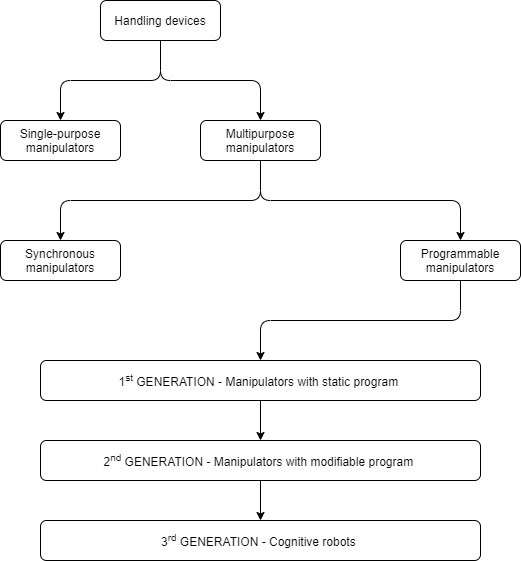
\includegraphics[width=0.8\linewidth]{img/manipulators.jpg}
    \caption{Classification of handling devices \cite{vsb_2007}}
    \label{fig:manipulators}
\end{figure}

\begin{itemize}

    \item  single-purpose manipulators -- characterized by limited movement possibilities, level of control suitable for the application, design and drives corresponding to the equipment being operated and the technology being used, 

    \item multipurpose manipulators -- they are multipurpose with the possibility of adapting to different technologies. The choice between single-purpose and universal industrial robots and manipulators is based on the overall assessment of the technology, workplace, etc., and must respect both the technical and economic aspects,

    \item  synchronous manipulators -- control is performed continuously by a human. These handling mechanisms are amplification devices for amplifying the force and motion variables on based on stimuli triggered by a human. They are independent of the machine being operated. The manipulator and the human form a closed control loop. These devices transmit human commands remotely. This possibility of remote control was used for scientific, medical and military purposes. Even today, some operations are carried out indirectly using miniature manipulators, 

    \item  programmable manipulators -- they are controlled by a programming unit,

    \item  programmable manipulators with fixed program -- the program does not change during the operation of the handling mechanism, it is fixed, the programming unit is of simple design, 

    \item  programmable manipulators with modifiable programs -- they have the possibility of switching or selecting the program, usually according to the scene in which the manipulators are currently in. These are usually devices with adaptive control. They are currently at the cutting edge of design and we call them industrial robots,

    \item  cognitive robots -- robots equipped with the ability to perceive and think rationally \cite{vsb_2007}.

\end{itemize}

\section{Industrial robots}

A robot is an automatically or computer-controlled integrated system capable of autonomous goal-oriented interaction with the natural environment according to instructions from a human. This
interaction consists of:

\begin{itemize}

    \item in the perception and recognition of that environment,
    \item manipulating objects or moving around in this environment. 

\end{itemize}

 Industrial robots are of more complex design than other handling devices and differ from other handling mechanisms primarily in the level of control.  Industrial robots are characterised by the following features:
 
\begin{itemize}
 
    \item  manipulation capability, i.e. grasping and moving objects, 
    \item behavioural autonomy, i.e. a complex sequence of actions performed automatically according to a specific program. Of particular importance is the case where this program is not fixed (given by design, as in the case of classical automatic controllers) but modifiable,
    \item controlled either by a human or automatically by its own controller.  This makes it different from, e.g. teleoperators, which amplify and transmit motion commands remotely directly from the human, who is an integral part of the system,
    \item versatility in the sense of 'multipurpose', not 'omnipotence'. The devices do not serve a single purpose but for several, sometimes quite diverse, purposes. This is related to the possibility of changing the program,
    \item the existence of a link with the environment (perception). In addition to simple mechanical (touch) electromagnetic sensors, more complex systems can also include visual (using a television camera) and acoustic feedback,
    \item the spatial concentricity of the individual components (integration) is preferably (but not necessarily, if one of the components is a computer) into a single object. The consequence is, among other things, easy transportability. In some cases, the system may be required to be mobile \cite{vsb_2007}.

\end{itemize}

%% The classification

\section{Classification of industrial robots and their structures}

Industrial robots can be classified according to various criteria: the number of degrees of freedom, kinematic structure, drives used, workspace geometry, motion characteristics, control method, or programming method. According to the abovementioned criteria, several types of robots are distinguished:

\subsubsection*{Number of degrees of freedom}

\begin{itemize}
    \item universal robots -- six degrees of freedom,
    \item redundant robots -- more than six degrees of freedom,
    \item deficient robots -- less than six degrees of freedom.
\end{itemize}

\subsubsection*{Kinematic structure}

\begin{itemize}
    \item serial robots -- open-loop kinematic chain,
    \item parallel robots -- closed-loop kinematic chain,
    \item hybrid robots -- combining both types of kinematic chains.
\end{itemize}


\subsubsection*{Type of drives}

\begin{itemize}
    \item electric,
    \item hydraulic,
    \item pneumatic.
\end{itemize}

Currently, industrial robots with electric drives predominate in numbers. If high loads are required, hydraulic drives are used and for high speeds pneumatic drives are preferred.

\subsubsection*{Workspace geometry}

\begin{itemize}
    \item cartesian -- robotic arms equipped with three perpendicular linear axes,
    \item cylindrical -- robotic arms equipped with two linear axes and one rotary axis,
    \item spherical --  robotic arms equipped with two rotary axes and one linear axis,
    \item SCARA -- Selective Compliant Articulated Robotic Arm, also equipped with with two rotary axes and one linear axis but in a different configuration than a spherical robotic arm \cite{vsb_2007}.
\end{itemize}

\section{Industrial robotic arms programming}

Before we dive into the programming of industrial robotic arms, let us revise a few concepts.
A workcell represents a robot and a collection of machines or peripherals. A single robot controller is responsible for controlling the various appliances of a~ workcell.

A robot end effector is a peripheral placed at the end of the robotic arm. The~end effector represents the last link of the robot. According to the application, end effectors can be grippers, welding devices, spray guns, or grinding and deburring machines \cite{monkman_2007}.

The robot controller is equipped with a so-called interface software. The interface software makes it easier for the user to program the robotic arm.  
Two basic information need to be programmed into the robotic arm:

\begin{itemize}
    \item position data -- i.e., where the robotic arm has to move to,
    \item procedure -- i.e., what action the robotic arm will perform at the specific position.
\end{itemize}

A robot position can be taught in several different ways:

\begin{itemize}
    \item positional commands -- the programmer inputs the position data using a GUI or text-based commands,
    
    \item Online programming, which is further divided into two types:
    
    \begin{itemize}
    
    \item pendant -- the pendant is a handheld control and programming unit attached to the robot controller,
    \item lead-by-the-nose -- the robotic arm is de-energized and moved along the required positions by hand while the robotic controller saves them into memory.
    
    \end{itemize}
    
    \item offline programming -- the robotic cell including the robotic arm and machines are represented in a specialized software. The robot can be moved in the software and brand-specific applications for the robotic controller can be created \cite{robodkmethods}.
  

\end{itemize}

\subsection{Offline programming}
Different robot brands have incompatible interfaces. Robot programming languages evolve slowly, and robot manufacturers offer backwards compatibility. For example, FANUC uses not one, but two programming languages for their controllers: 

\begin{itemize}

 \item TP language -- suitable for programming position data,
 \item KAREL language -- high-level language based on Pascal, suitable for programming logical constructs \cite{fanuchandling}.

\end{itemize}

Offline programming  (OLP) refers to a programming method in which the robot is programmed outside the production environment. OLP helps to eliminate production downtime and allows studying multiple scenarios of a robot cell before setting up the production cell. OLP also aids in predicting mistakes made in designing a workcell. The OLP workflow can be summarized into the following steps:

\begin{enumerate}
  \item creating/importing a robotic cell that mimics the real life workcell,
  \item importing a CAD file representing the machined part,
  \item programming (graphical or textual) and automatic generation of robot path,
  \item simulation and validation -- collision detection, join violations etc.,
  \item reporting -- efficiency, productivity, cycle time etc.,
  \item translating the robot program for a specific controller using a post processor,
  \item executing the robot program in a actual workcell \cite{offlinesteps}.
\end{enumerate}
